Given the size of the data our software will be working on, it requires an efficient way of storing them.

There are 2 kinds of data, on the first hand the parameters and utilities ; on the other hand, the ones the programs works on.
\subsection{Boards and node}
Boards are stored as bitboard. As the game is played on a 8x8 board, it is convinient to use a 64 bit integer to store the positions of the pieces.
That way, each and every of a kind of pieces are stored on the same integer, saving space compared to a matrix 8 x 8.
Players own rabits, cats, dogs, horses, camel and elephant; thus using 6 integer for each player do the job. Adding an additionnal bitboard to store the position of every pieces of each players helps to increase the speed of the algorithm by reducing the number of test required to be done during the playout phases.

Nodes are stored in an array, thus grouping them on a countinous memory segment. Therefore the time to gain access to them is increased.
They also countains statistics, a pointer to its parent, a pointer to the first of their children and the number of children they own.

\begin{figure}[!h] 
\centerline{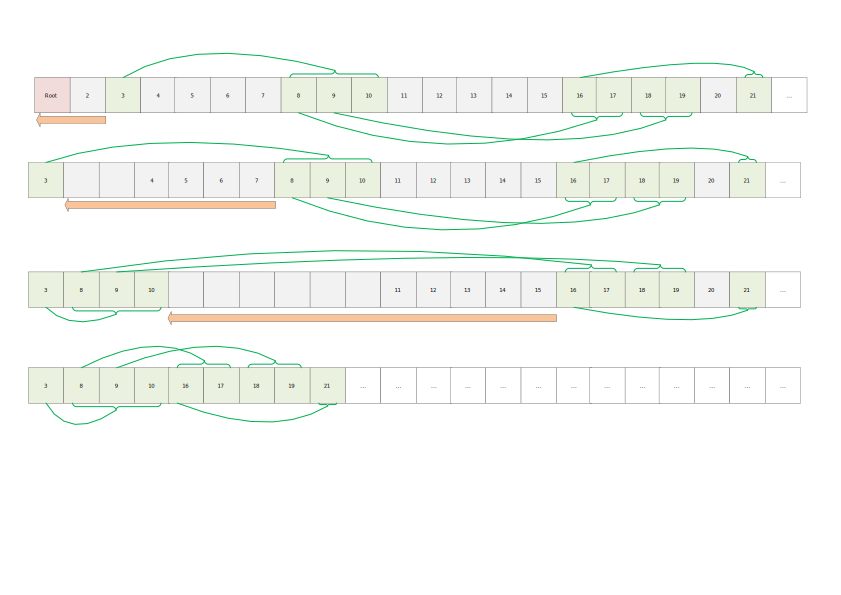
\includegraphics[scale=0.70]{Data_Structure/Img/array.png}}
\caption{\label{fig:array}\textit{Prunning of the tree}.}
\end{figure}
In order to prune the tree, we use the following method : create a copy of the current tree (\_tree) into a buffer (\_buff).
The root of the buffer tree will be a copy the chosen node. Then the children are saved following the branches. The advantage of this method is that you only copy the nodes you want to keep.
However the memory used of the buffer need to be the same as the one of the tree before the prunning. Thus the maximum memory that can be used by the tree (\_tree) is half the memory used by the program.
In order to dermine the number of leaves to be created, the program check how much memory there is left on the computer and use 90\% of it.

%\ensuremath{\fract{RAM \times 90\%}{2} = Number of leaves}

\subsection{Utilities and parameters}
